\documentclass[12pt,a4paper]{book}
\raggedbottom

\usepackage{ugmath}
\usepackage{float}
\usepackage{placeins}
\usepackage[labelfont=bf,labelsep=space]{caption}
\usepackage{pdfpages}


\begin{document}


    \thispagestyle{empty}
    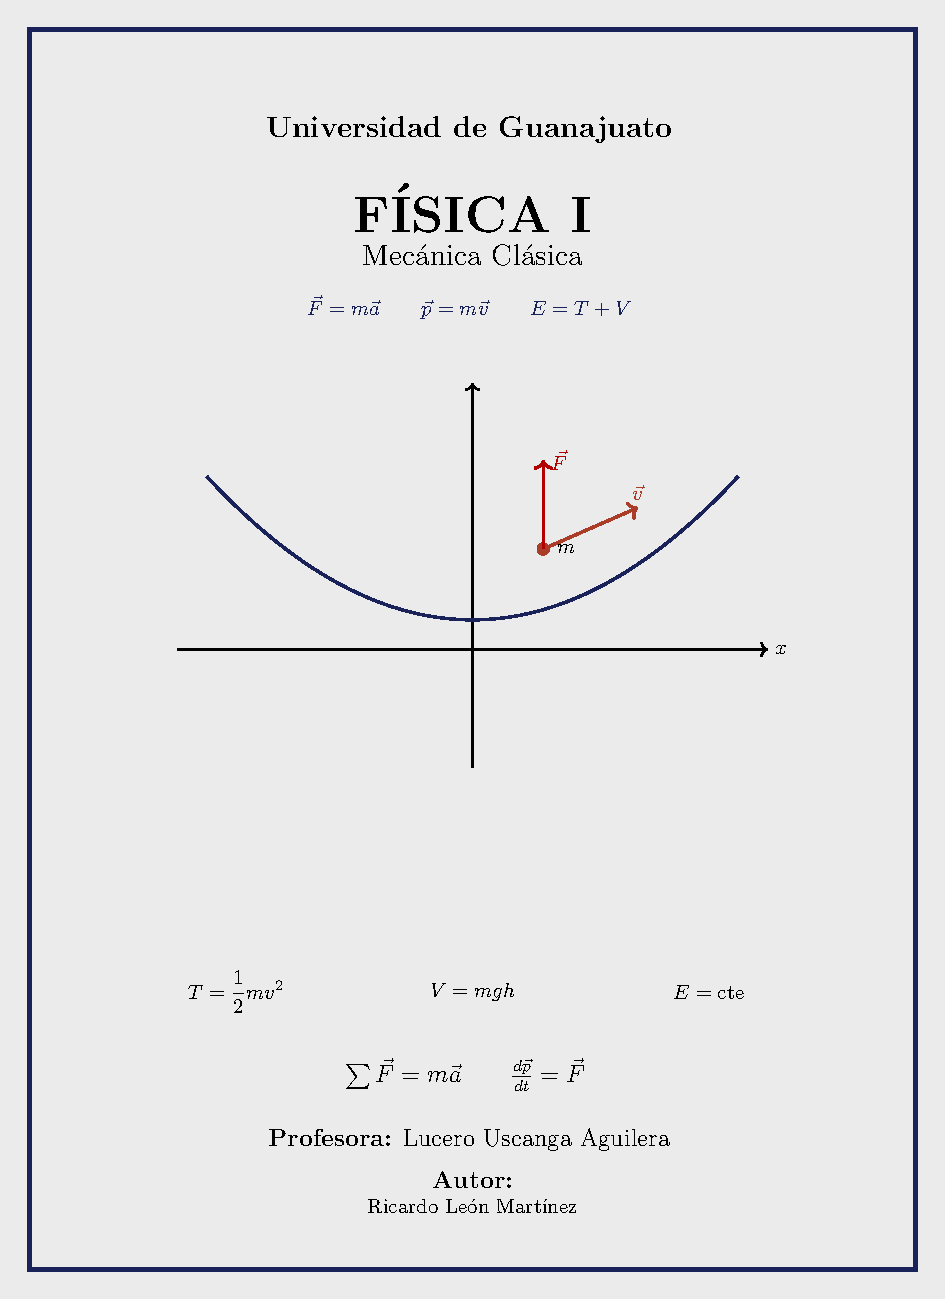
\includepdf[pages=1]{Figura.pdf}
    

    \setcounter{page}{1}
    \tableofcontents
    \clearpage

    \chapter{Introducción}

    \section{¿Qué es la física?}

    La palabra física proviene del término griego $\phi\upsilon\sigma\iota\zeta$ que significa \textbf{naturaleza}, y por ello la física
    debía ser una ciencia dedicada al estudio de todos los fenómenos naturales. Especificamente, la física es una ciencia cuyo objetivo
    es estudiar los componentes de la materia y sus interacciones mutuas.

    \section{Partes clásicas de la física}

    Al principio los sentidos del ser humano fueron las fuentes de informacion de ellos clasificó los fenómenos observados de acuerdo a la manera
    en la que los percibía.\\
    La \textbf{luz} fue relacionada con la \textbf{visión} y la \textbf{óptica} se desarrolló como una ciencia más o menos independiente relacionada
    a ella. El \textbf{sonido} fue relacionado con la \textbf{audición} y la \textbf{acústica} se desarrolló como ciencia correlativa. El \textbf{calor}
    fue relacionado con otra sensación física, y por muchos años el estudio de calor (denominado \textbf{termodinámica}) fue otra parte autónoma
    de la física. El \textbf{movimiento}, es el más común de todos los fenómenos observados directamente, y la ciencia del movimiento, la \textbf{mecánica},
    se desarrolló mas temprano que cualquier otra rama de la física. Por ejemplo, el movimiento de los planetas causado por sus interacciones gravitatorias,
    así como la caída libre de los cuerpos, fue satisfactoriamente explicado por las leyes de la mecánica; por ello la \textbf{gravitación} se considero
    tradicionalmente como un capitulo de la mecánica. El \textbf{electromagnetismo}, no estando relacionado directamente con ninguna experiencia sensorial,
    no aparecio como una rama de la fisica sino hasta el siglo XIX. De esta manera en el siglo XIX la física aparecía dividida en unas pocas ciencias o ramas
    (llamadas clásicas): \textbf{mecánica}, \textbf{termodinámica}, \textbf{acústica}, \textbf{óptica}, \textbf{electromagnetismo}. La mecánica fue con toda
    propiedad, el principio guía para todas ellas. Los desarrollos de la física del XX están comprendidos en la denominada \textbf{física moderna}.
    Es importante señalar que, la física será siempre un todo que debe considerarse de una manera lógica y consecuente.

    \section{Nuestra visión del Universo}

    La materia está compuesta por partículas fundamentales (o elementales) y que todos los cuerpos vivientes e inertes están hechos de diferentes grupos de
    ordenamiento de tales partículas. Tres de estas partículas fundamentales son: \textbf{electrones}, \textbf{protones}, \textbf{neutrones}. Existe otras
    partículas, cuya vida es transitoria, se crean y destruyen continuamente. Su existencia se manifiesta mediante técnicas de observación eleboradas. Usando
    un lenguaje muy simplificado, podemos decir que las tres partículas, el electrón, el protón y el neutrón, están presentes en grupos bien definidos llamados
    \textbf{átomos}, con los protones y los neutrones situados en una región central muy pequeña denominada núcleo. Se han reconocido cerda de $104$ "especies"
    diferentes de átomos, pero hay alrededor de 1300 "variedades" diferentes de átomos, denominados \textbf{isótopos}. Los átomos a su vez forman otros agegados
    llamados \textbf{moléculas}, de las cuales se sabe que existen varios millones. El número de moléculas diferentes es muy grande, ya que día a día más y más
    moléculas se sintetizan en los laboratorios de química. Finalmente, las moléculas se agrupan formando cuerpos (o materia en conjunto) apareciendo como sólidos,
    líquidos o gases, aunque esta clasificación no es del todo rígida. El cuerpo humano es el más desarrollado de los entes vivientes, está compuesto de $10^{28}$
    \textbf{átomos}; la mayor parte de los cuales son átomos de \textbf{C}, \textbf{H}, \textbf{O} y \textbf{N}. El sistema solar es un conjunto de varios cuerpos
    llamados \textbf{planetas}, los cuales giran alrededor de una estrella, denominada \textbf{sol}. Uno de esos planetas es nuestra Tierra, la cual contiene cerca
    de $10^{51}$ \textbf{átomos}. El sol está compuesto de cerca de $10^{57}$ \textbf{átomos}. El sistema solar es a su vez una pequeña parte de un gran agregado
    de estrellas que forman una galaxia llamada la \textbf{Vía Láctea}, compuesta de cerca de $10^{11}$ \textbf{estrellas} o $10^{70}$ \textbf{átomos} y con una
    forma de disco, con un diametro de $10^{21}m$ o alrededor de \textbf{100000} años luz y un espesor máximo de $10^{20}m$. Se han observado muchas galaxias
    similares a la nuestra, estando la más cercana a \textbf{dos millones} de años luz de nosotros. El universo puede contener $10^{20}$ \textbf{estrellas}, agrupadas
    en cerca de $10^{10}$ \textbf{galaxias}. Algunas preguntas vienen naturalmente a nuestra mente: ¿Por qué y cómo se unen los electrones, protones y neutrones
    para formar atomos?, ¿Por qué y cómo se unen los átomos para formar moléculas?, ¿Por qué y cómo las moléculas se unen para formar cuerpos?, ¿Cómo es que la materia
    se agrega para formar desde partículas de polvo hasta planetas gigantes, desed bacterias hasta esa criatura maravillosa que es el hombre? Nosotros podemos
    responder en principio estas preguntas fundamentales, introduciendo la noción de \textbf{interacción}. Por ejemplo, decimos que las partículas de un átomo
    interactúan entre sí, a modo de producir una configuración estable. Los átomos a su vez interactuan para formar cuerpos. La materia en conjunto tambien exhibe
    ciertas interacciones obvias, tales como la gravitación. El objetivo primario del físico es descubrir las diferentes interacciones de la materia; éstas son
    principalmente interacciones \textbf{gravitaciones}, \textbf{electromagnetica} y \textbf{nucleares}. El físico trata luego de expresarlas en una manera
    cuantitativa, para lo cual requiere de las matemáticas. Finalmente, intenta formular reglas generales acerca del comportamiento de la materia en conjunto -
    comportamiento que resulta de estas interacciones fundamentales. La física cubre rangos tremendos de magnitudes, yendo desde longitudes del orden de
    $10^{-15}m$ y masas del orden de $10^{-31}kg$ (correspondientes a una sola partícula tal como el electrón), hasta - y aun mas alla de - longitudes del
    orden $10^{30}kg$ (correspondiente a cuerpos de nuestro sistema solar).

    \section{Relación de la física con otras ciencias}

    El objetivo de la física es capacitarnos para comprender los componentes básicos de la materia y sus interacciones mutuas, y explicar así los fenómenos naturales,
    incluyendo las propiedades de la materia en conjunto. Por tanto , la física es la más fundamental de todas las ciencias naturales. Por ejemplo, la química trata
    básicamente un aspecto particular de este ambicioso programa: la aplicación de las leyes de la física a la formación de las moléculas y los variados métodos
    prácticos de tranformación de ciertas moléculas en otras. La física es importante porque proporciona la base conceptual y la estructura teórica sobre la cual
    se fundan las otras ciencias naturales. Desde el punto de vista práctico es importante porque proporciona técnicas que pueden utilizarse casi en cualquier
    área de la investigación pura o aplicada. Por ejemplo, eñ astrónomo requiere de técnicas ópticas, de radio y espectroscópicas.

    \chapter{Fuerzas}

    La definición precisa de fuerza se analizara en el tema siguiente, cuando veamos la dinámica del moviemiento y las leyes de Newton. Ahora estudiaremos la composición de fuerzas
    y en particular el equilibrio de ellas (\textbf{Estática}), un problema de gran aplicación en la ingenieria. \textbf{Fuerza = cantidad vectorial con magnitud y dirección}.
    Es costumbre en ingenieria, cuando se hace referencia a libras-fuerzas y a kilogramos-fuerza, es decir, simplemente "libras" y "kilogramos", aunque estos términos realmente
    corresponden a unidades de masa.

    \section{Composición de fuerzas}

    \begin{mdframed}[style=mdbluebox,frametitle={Definición 1: Fuerzas concurrentes}]
        Se dice que una fuerza es concurrente o que las fuerzas se estan aplicando en el mismo punto, si la resultante es el vector suma
        \begin{equation*}
            \vec{R}=\vec{F}_{1}+\vec{F}_{2}+\cdots+\vec{F}_{n}=\sum_{i=1}^{n}\vec{F}_{i}.
        \end{equation*}
    \end{mdframed}

\end{document}